
\section{Deciphering Latent CoT Reasoning: An Information-Theoretic View}
\label{sec:info_theory}

While Section~\ref{sec:process_supervision} establishes the efficacy of trajectory supervision and space supervision, a critical uncertainty remains regarding the internal mechanics: \textit{how do varying training paradigms and constraints shape the semantic content of these continuous hidden states?}~\citet{zhang2025latenttokensthinkcausal} caution that without explicit grounding, latent tokens may function merely as uninterpretable placeholders or robust shortcuts rather than faithful encoders of causal reasoning.
To resolve this ambiguity and rigorously characterize the nature of the encoded information, we move \textit{beyond surface-level performance} metrics and adopt an information-theoretic lens.

\begin{figure}[t]
    \centering
    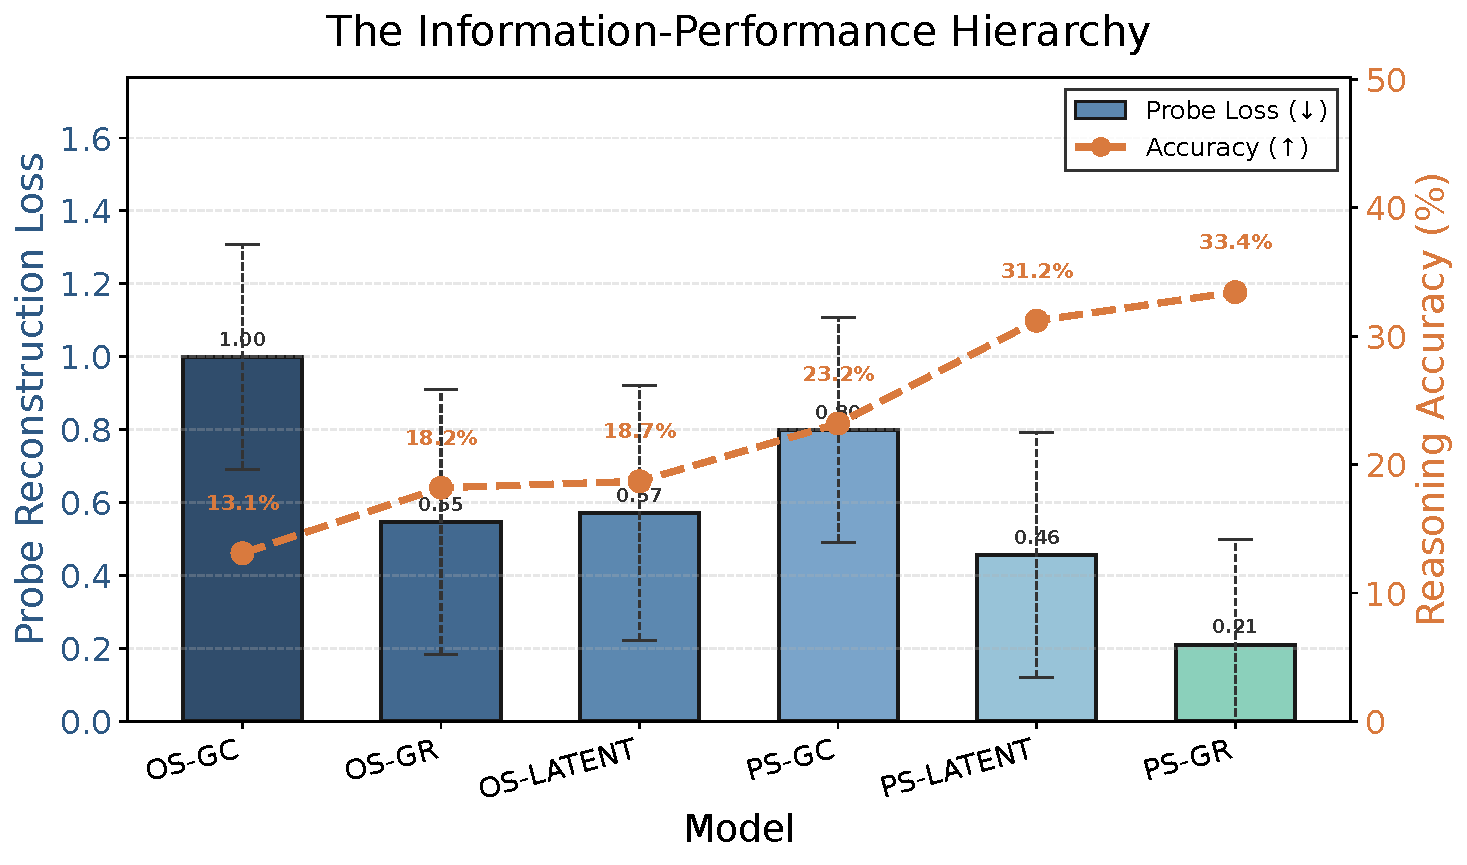
\includegraphics[width=\linewidth]{Figures/Fig3/probe_loss_acc_dual.pdf} 
    \caption{Information-performance hierarchy with ULP loss and relevant performance across different paradigms. }
    \label{fig:info_hierarchy}
\end{figure}

\paragraph{Variational Information Bounds for Latent CoT}
\label{sec:mi_estimation}

While the ultimate theoretical objective is to maximize mutual information with the final answer, direct estimation is intractable. Consequently, we pivot to a step-wise proxy. Let $S_t$ denote the ground-truth explicit reasoning step at time $t$. 
Crucially, we posit that $S_t$ somehow aligns with the proper semantic direction of the reasoning process, serving as the immutable reference for the latent state $L_t$.
We quantify the quality of the latent representation by estimating the mutual information $I(L_t; S_t)$:
\begin{equation}
    I(L_t; S_t) = H(S_t) - H(S_t \mid L_t)
\end{equation}
Since the marginal entropy of the ground truth $H(S_t)$ is constant for a fixed dataset, maximizing $I(L_t; S_t)$ is equivalent to minimizing the conditional entropy $H(S_t \mid L_t)$.

To address the intractability of computing $H(S_t \mid L_t)$ for continuous variables, we introduce a \emph{variational upper bound} using a parametric probe $q_{\phi}(S_t\mid L_t)$. This probe acts as a lightweight decoder approximating the true posterior distribution. Its expected negative log-likelihood serves as a rigorous proxy for the conditional entropy:
\begin{equation*}
    \mathcal{L}_{\text{Info}}(L_t, S_t) = \mathbb{E}_{L_t \sim \pi} [-\log q_{\phi}(S_t \mid L_t)] \geq H(S_t \mid L_t)
\end{equation*}
where $\pi$ represents the frozen policy of the model being evaluated.
We freeze the best-performance checkpoints of all baselines and train a single \emph{Unified Latent Probe (ULP)} architecture on their generated latent states (See Appendix~\ref{app:d} for detailed training setting and curves.). The converged reconstruction loss $\mathcal{L}_{\text{Info}}$ thus provides a quantitative metric for semantic fidelity: a lower $\mathcal{L}_{\text{Info}}$ corresponds to a tighter upper bound on conditional entropy, directly implying a higher lower bound on MI.
From an optimization perspective, this establishes a direct correspondence between \textit{reconstructibility} and \textit{learnability}: latent states with low $\mathcal{L}_{\text{Info}}$ indicate that the model has successfully captured the rigorous semantic direction of the explicit logic, whereas high reconstruction error signals a divergence into high-entropy regions.

\paragraph{The Information Hierarchy: Scaffolding as Mutual Information Maximization}
\label{subsec:info_hierarchy}


\begin{figure}[t]
    \centering
    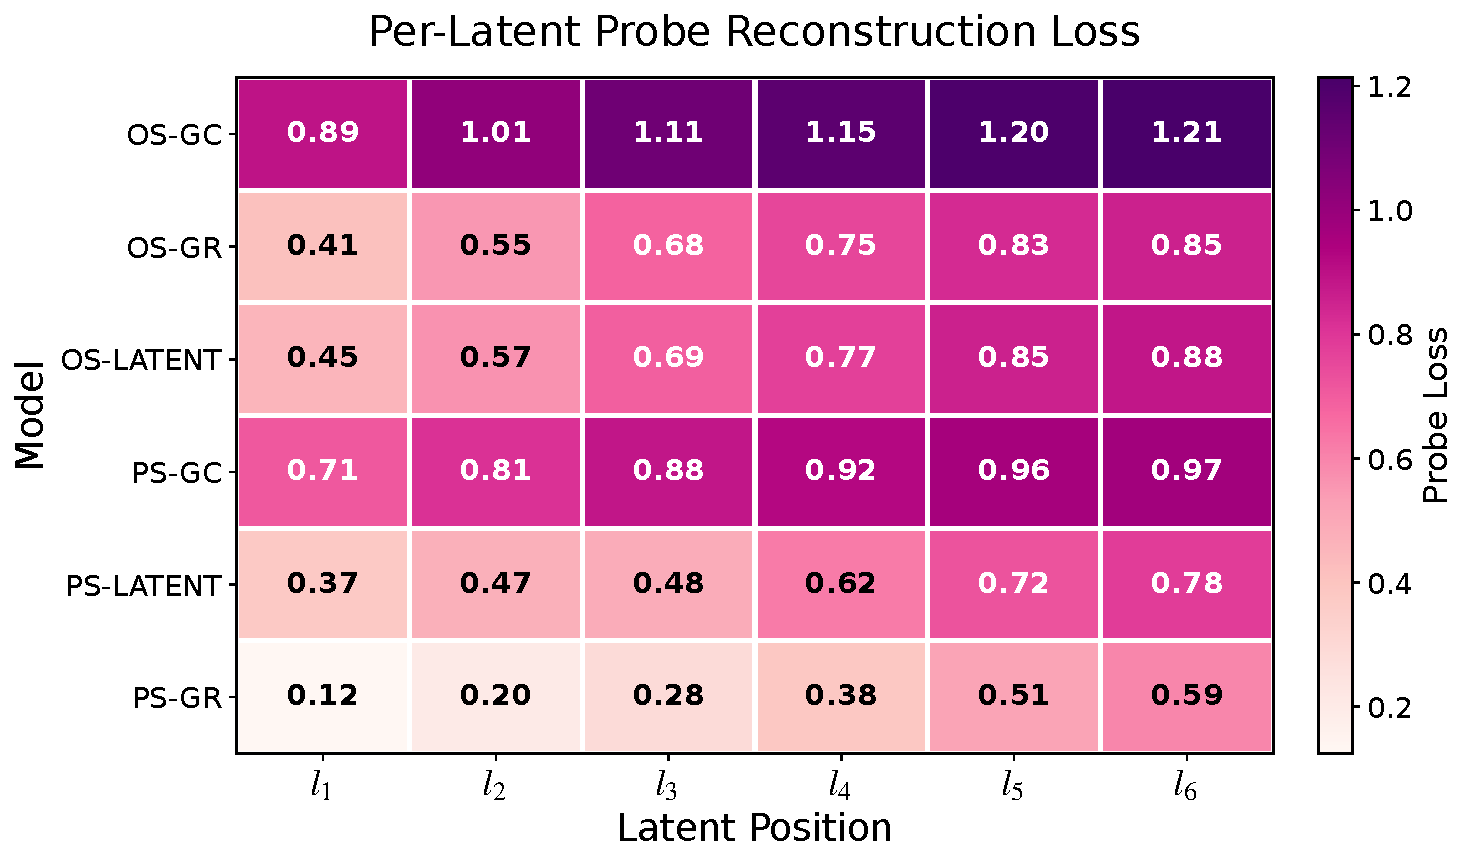
\includegraphics[width=\linewidth]{Figures/Fig3/probe_loss_per_latent_heatmap.pdf} 
    \caption{Spatiotemporal information decay, with visualization of step-wise ULP loss across the latent trajectory ($L_1 \to L_6$). A universal phenomenon of \textit{information decay} is observed as the reasoning chain lengthens.}
    \label{fig:info_decay}
\end{figure}

Figure~\ref{fig:info_hierarchy} visualizes the ULP loss $\mathcal{L}_{\text{Info}}$ alongside reasoning performance. The results reveal a striking \textbf{information hierarchy}, characterized by a rigorous inverse correlation where reasoning accuracy is strictly upper-bounded by the fidelity of information retention.
\textsc{OS-variants} exhibit consistently high reconstruction losses, indicating a fundamental absence of reasoning-critical semantics within their latent states. Since the probe cannot extract valid logic, we infer that the optimization degenerates into encoding uninterpretable shortcut features. Even for \textsc{OS-GR}, which explicitly adds a reconstruction objective, fails to bridge this gap. 
This suggests that without the \textit{causal logical signals}, the reconstruction loss alone is insufficient to locate the correct reasoning manifold.

Moving to \textsc{PS-Latent}, we observe a significant drop in probe loss even \textit{without space supervision}. This validates the theoretical impact of trajectory supervision: by optimizing the local stepwise objective $I(L_{\le t}; S_{t+1})$, the training process inherently constrains the latent manifold to be predictive of the immediate reasoning step. This causal pressure forces the continuous states to retain significant semantic information to satisfy the next-token prediction requirement.
Building upon this foundation, \textsc{PS-GR} achieves the optimal frontier. By introducing the generative decoding objective, it maximizes the variational lower bound of $I(L_t; S_t)$. This ensures that the model \textit{internalizes} the scaffolding, transmuting the explicit rationale into a \textit{semantics-preserving latent format that retains full logical fidelity}. \textsc{PS-GC} also suffers from severe information decay because its rigid Euclidean alignment functions as a \textit{destructive constraint}, forcing the high-dimensional reasoning manifold to collapse onto static embeddings, thereby obliterating the fine-grained semantic fidelity required for reconstruction.

To dissect the spatio dynamics of reasoning, Figure~\ref{fig:info_decay} tracks the evolution of ULP loss across the latent trajectory. We observe a universal phenomenon of \emph{information decay}, where reconstruction error progressively accumulates as the chain lengthens. 
This reflects an inherent vulnerability of autoregressive latent generation: unlike training under teacher forcing, where ground-truth signals correct deviations at every step, inference allows minor errors to cascade, driving the trajectory into high-entropy regions.
This decay is catastrophic for unaligned or geometrically constrained baselines, which suffer from rapid semantic collapse as their states drift effectively detached from the logical path. 
In this context, the generative reconstruction objective functions as a crucial recurrent calibration mechanism. By enforcing reconstructibility at each transition, it effectively ``resets'' the accumulating semantic drift, distilling noisy hidden states back into clear, calibrated units that ensure the entire trajectory remains a faithful carrier of the reasoning process.